\documentclass[a4paper,12pt]{article}

\usepackage{graphicx}
\usepackage{caption}
\usepackage{subcaption}
\usepackage[utf8]{inputenc}
\usepackage[english,greek]{babel}
\usepackage{hyperref}

\title{Τεχνικές Βελτιστοποίησης - Εργασία 2}
\author{Ρουσομάνης Γεώργιος (ΑΕΜ: 10703)}
\date{Νοέμβριος 2024}

\begin{document}

\maketitle

\section*{Εισαγωγή}

Ο στόχος της παρούσας εργασίας είναι η ελαχιστοποίηση μιας συνάρτησης πολλών μεταβλητών χωρίς περιορισμούς με 
τη χρήση παραγώγων και η μελέτη της αποτελεσματικότητας διαφορετικών αλγορίθμων βελτιστοποίησης. Ειδικότερα,
η αντικειμενική συνάρτηση που θα εξεταστεί είναι:

\[
f(x, y) = x^5 e^{-x^2 - y^2}.
\]

Οι μέθοδοι που θα χρησιμοποιηθούν για την αναζήτηση του ελαχίστου περιλαμβάνουν:
\begin{itemize}
    \item \textbf{Μέθοδος Μέγιστης Καθόδου \selectlanguage{english} (Steepest Descent) }
    \item \textbf{Μέθοδος \selectlanguage{english} Newton}
    \item \textbf{Μέθοδος \selectlanguage{english} Levenberg-Marquardt}
\end{itemize}

Η κατεύθυνση καθόδου $d_k$ καθορίζεται διαφορετικά σε κάθε μέθοδο, ενώ το βήμα $\gamma_k$ μπορεί να επιλεχθεί
είτε σταθερό, είτε με ελαχιστοποίηση της $f(x_k + \gamma_k d_k)$, είτε βάσει του κανόνα 
\selectlanguage{english} Armijo. \selectlanguage{greek}
Σε κάθε επανάληψη, το νέο σημείο υπολογίζεται ως $x_{k+1} = x_k + \gamma_k d_k$
ενώ οι αλγόριθμοι τερματίζουν όταν $|\nabla(x_k)| < \epsilon$ όπου $\epsilon > 0$. 

Στόχος είναι να μελετηθούν και να συγκριθούν οι παραπάνω αλγόριθμοι, τόσο ως προς την αποδοτικότητά 
τους όσο και ως προς τον αριθμό επαναλήψεων που απαιτούνται για την σύγκλισή τους. Παράλληλα, 
θα εξεταστούν η επίδραση του σημείου εκκίνησης $(x_0, y_0)$ καθώς και η επιλογή του βήματος $\gamma_k$ 
στη σύγκλιση και την αποδοτικότητα του κάθε αλγορίθμου.

Τέλος, θα διερευνηθούν οι περιπτώσεις όπου οι μέθοδοι δεν καταλήγουν στο σωστό αποτέλεσμα, προσδιορίζοντας 
πιθανούς λόγους όπως εγκλωβισμό σε τοπικά άκρα.

\section*{Μέθοδος Μέγιστης Καθόδου}
Σε αυτή τη μέθοδο, το διάνυσμα κατεύθυνσης $d_k$ επιλέγεται ως $d_k = -\frac{\nabla f(x_k)}{|\nabla f(x_k)|}$.
Η χρήση του μοναδιαίου διανύσματος για το $d_k$ εξασφαλίζει ότι το διάστημα αναζήτησης κατά την ελαχιστοποίηση της $f(x_k + \gamma_k d_k)$ εκφράζεται σε φυσικές μονάδες, διατηρώντας έτσι τη συμβατότητα των υπολογισμών με το 
πρόβλημα βελτιστοποίησης. Ένα επιπλέον πλεονέκτημα της κανονικοποίησης του $d_k$ είναι ότι, σε σημεία όπου η 
κλίση είναι πολύ μικρή, το διάστημα αναζήτησης και το βήμα $\gamma_k$ παραμένουν μικρά, οδηγώντας σε μικρότερα 
βήματα και συνεπώς σε περισσότερες επαναλήψεις. Ενώ η μέθοδος μέγιστης καθόδου μας παρέχει ισχυρή εγγύηση για την
σύγκλισή της, δεν είναι υπολογιστικά αποτελεσματική όπως θα διαπιστώσουμε στη συνέχεια.

\subsection*{Σταθερό βήμα}
Στο Σχήμα~\ref{fig:gradient_descend_fixed_step_contour} παρατηρούμε τα διαδοχικά σημεία που υπολογίζει ο αλγόριθμος
σε κάθε επανάληψη για $\gamma_k = 0.001$. Είναι σημαντικό να τονίσουμε ότι στην περίπτωση του σταθερού βήματος 
το $\gamma_k$ πρέπει να είναι αρκούντως μικρό διαφορετικά μπορεί να υπάρξει αδυναμία σύγκλισης ή ταλαντώσεις.

Προφανώς για το αρχικό σημείο $(0,0)$ ισχύει $\nabla f = 0$, επομένως ο αλγόριθμος τερματίζει αμέσως.
Για το $(-1, 1)$ έχουμε επιτυχή σύγκλιση καθώς βρισκόμαστε αρκούντως κοντά στο ολικό ελάχιστο. Ωστόσο για το
$(1, -1)$ έχουμε αδυναμία σύγκλισης λόγω της επίπεδης επιφάνειας που εισέρχεται η μέθοδος όπου $\nabla f \approx 0$.
Όπως θα δούμε στην συνέχεια το πρόβλημα αυτό αίρεται με την ελαχιστοποίηση της $f(x_k + \gamma_k d_k)$ ή 
με τον κανόνα \selectlanguage{english} Armijo.

\selectlanguage{greek} Επίσης παρατηρούμε ότι η τροχιά που
διαγράφουν τα διαδοχικά σημεία που υπολογίζει ο αλγόριθμος είναι κάθετη στις ισοδυναμικές επιφάνειες. Αυτό
συμβαίνει επειδή το $d_k$ έχει την κατεύθυνση της μέγιστης μείωσης της συνάρτησης, και σε κάθε σημείο πάνω στην 
ισοδυναμική επιφάνεια η συνάρτηση παραμένει σταθερή, άρα η παράγωγος της συνάρτησης σε κάθε κατεύθυνση πάνω στην
επιφάνεια είναι μηδέν. 

Στο Σχήμα~\ref{fig:gradient_descend_fixed_step_costs} φαίνεται η σύγκλιση της μεθόδου
σε κάθε επανάληψη για τα αρχικά σημεία $(-1, 1)$, $(1, -1)$.

\begin{figure}[h]
    \centering
    \begin{minipage}{0.47\textwidth} % Ορίζει το πλάτος της πρώτης εικόνας
        \centering
        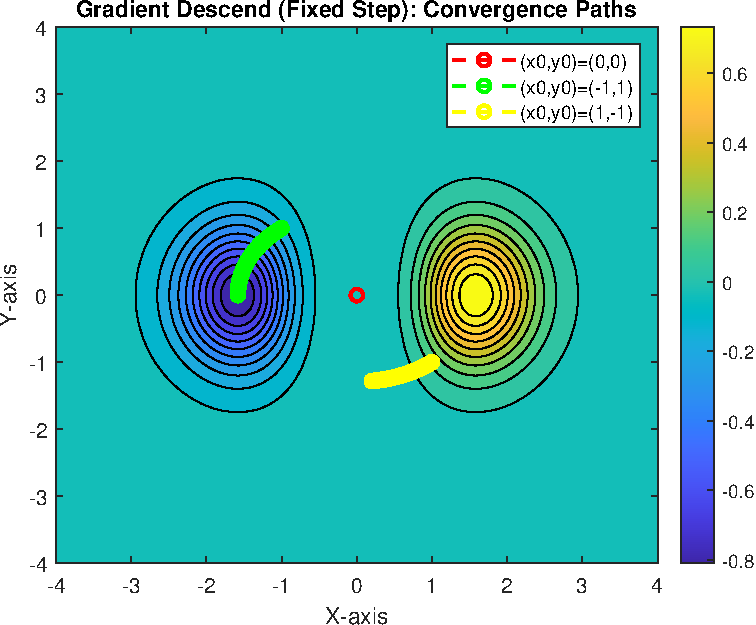
\includegraphics[width=1\linewidth]{plot/gradient_descend_fixed_step_contour.pdf}
        \caption{\small Διαδοχικά σημεία υπολογισμού της μεθόδου Μέγιστης Καθόδου για σταθερό βήμα $\gamma_k=0.001$}
        \label{fig:gradient_descend_fixed_step_contour}
    \end{minipage} \hfill
    \begin{minipage}{0.47\textwidth} % Ορίζει το πλάτος της δεύτερης εικόνας
        \centering
        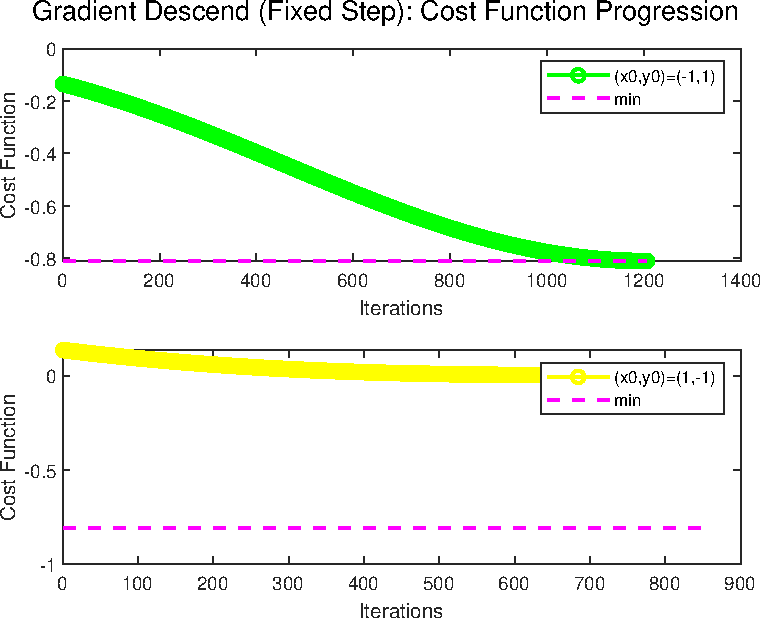
\includegraphics[width=1\linewidth]{plot/gradient_descend_fixed_step_costs.pdf}
        \caption{\small Σύγκλιση της μεθόδου Μέγιστης Καθόδου για σταθερό βήμα $\gamma_k=0.001$}
        \label{fig:gradient_descend_fixed_step_costs}
    \end{minipage}
\end{figure}

\subsection*{Βήμα με ελαχιστοποίηση}
Σε αυτή την περίπτωση θα υπολογίσουμε το $\gamma_k$ που ελαχιστοποιεί την $f(x_k + \gamma_k d_k)$ σε ένα προκαθορισμένο
διάστημα αναζήτησης $d$. Για τον σκοπό αυτό θα χρησιμοποιήσουμε την μέθοδο \selectlanguage{english} Fibonacci.
\selectlanguage{greek} Πρόφανώς για να συγκλίνει η μέθοδος \selectlanguage{english} Fibonacci \selectlanguage{greek} 
στο ελάχιστο θα πρέπει η συνάρτηση να είναι αυστηρά σχεδόν κυρτή στο $d$. Επίσης για το αρχικό σημείο $(1, -1)$, 
το $d$ πρέπει να είναι αρκούντως μεγάλο ώστε να ξεπεράσουμε την περιοχή όπου $\nabla f \approx 0$. Στο 
Σχήμα~\ref{fig:gradient_descend_line_minimization_contour}
παρατηρούμε ότι η μέθοδος συγκλίνει για τα αρχικά σημεία $(-1, 1)$, $(1, -1)$. Επίσης βλέπουμε ότι η πορεία προς το 
ελάχιστο είναι μία τεθλασμένη γραμμή, με τα διαδοχικά ευθύγραμμα τμήματα να είναι κάθετα μεταξύ τους, όπως αναμέναμε
άλωστε από την θεωρία. Από το Σχήμα~\ref{fig:gradient_descend_line_minimization_costs} φαίνεται πως η σύγκλιση για 
αρχικό σημείο $(-1, 1)$ επιτεύθχει με πολύ μικρότερο αριθμό επαναλήψεων από ότι στην περίπτωση του σταθερού βήματος.

\begin{figure}[h]
    \centering
    \begin{minipage}{0.47\textwidth}
        \centering
        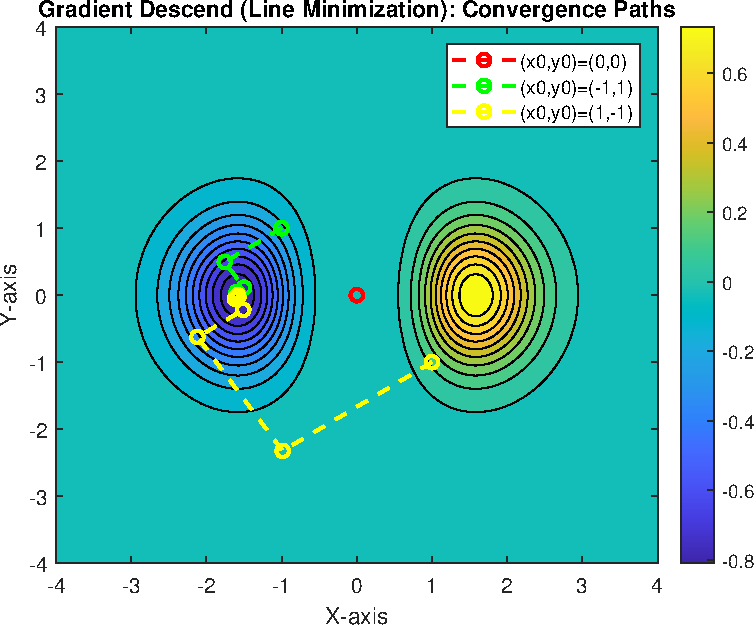
\includegraphics[width=1\linewidth]{plot/gradient_descend_line_minimization_contour.pdf}
        \caption{\small Διαδοχικά σημεία υπολογισμού της μεθόδου Μέγιστης Καθόδου για βήμα μέσω ελαχιστοποίησης}
        \label{fig:gradient_descend_line_minimization_contour}
    \end{minipage} \hfill
    \begin{minipage}{0.47\textwidth}
        \centering
        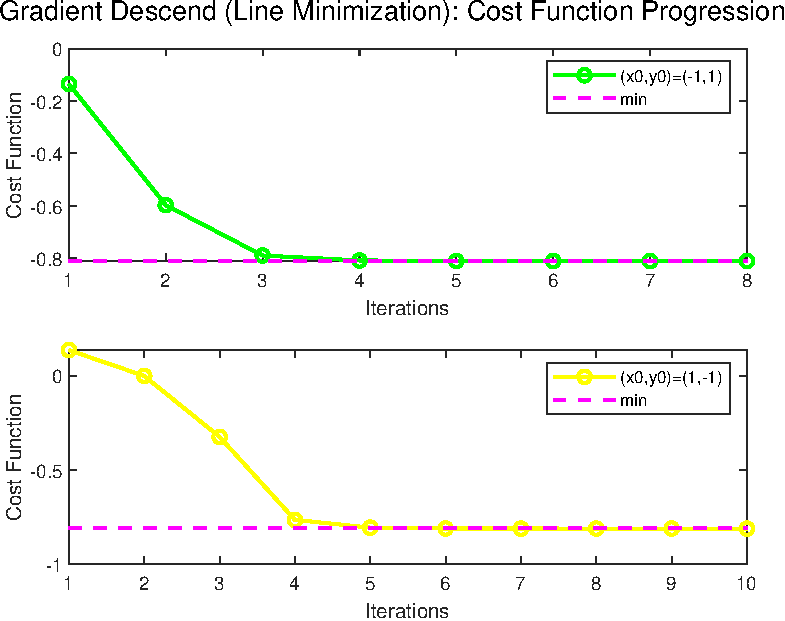
\includegraphics[width=1\linewidth]{plot/gradient_descend_line_minimization_costs.pdf}
        \caption{\small Σύγκλιση της μεθόδου Μέγιστης Καθόδου για βήμα μέσω ελαχιστοποίησης}
        \label{fig:gradient_descend_line_minimization_costs}
    \end{minipage}
\end{figure}

\subsection*{Βήμα με τον κανόνα \selectlanguage{english} Armijo}
\selectlanguage{greek}
Στο Σχήμα~\ref{fig:gradient_descend_armijo_rule_iters} παρουσιάζονται οι τρεις πρώτες επαναλήψεις της μεθόδου
\selectlanguage{english}Armijo\selectlanguage{greek} για τα αρχικά σημεία $(-1, 1)$ και $(1, -1)$,
με παραμέτρους $s = 3$, $\beta = 0.5$, και $\alpha = 0.01$. Οι τιμές των $\alpha$ και $s$ επιλέχθηκαν έτσι ώστε, 
στην πρώτη επανάληψη για το αρχικό σημείο $(1, -1)$, το $\gamma_k$ να είναι αρκετά μεγάλο για να αποφύγουμε την 
περιοχή όπου $\nabla f(x_k) \approx 0$.

Η αύξηση του $\alpha$ συνεπάγεται μεγαλύτερη κλίση της ροζ ευθείας (κατά απόλυτη τιμή), γεγονός που σημαίνει ότι η 
απαιτούμενη βελτίωση σε κάθε επανάληψη αυξάνεται. Η πράσινη ευθεία ορίζει τη μέγιστη δυνατή βελτίωση που μπορεί να 
επιτευχθεί και αντιστοιχεί σε τιμή $\alpha = 1$, ισούται δε με την κλίση της αντικειμενικής συνάρτησης στο υπό εξέταση
σημείο $x_k$.

Τέλος, η παράμετρος $\beta$ καθορίζει τον ρυθμό με τον οποίο μειώνεται το βήμα σε κάθε επανάληψη, επηρεάζοντας τη 
σταδιακή προσέγγιση της λύσης.

Από το Σχήμα~\ref{fig:gradient_descend_armijo_rule_costs} βλέπουμε ότι η μέθοδος μέγιστης καθόδου
με τον κανόνα\selectlanguage{english} Armijo \selectlanguage{greek} απαιτεί περίπου τον ίδιο αριθμό επαναλήψεων
με αυτόν της ελαχιστοποίησης συνάρτησης, συγκλίνει δε πολύ πιο γρήγορα από την περίπτωση σταθερού βήματος.


\begin{figure}
    \centering
    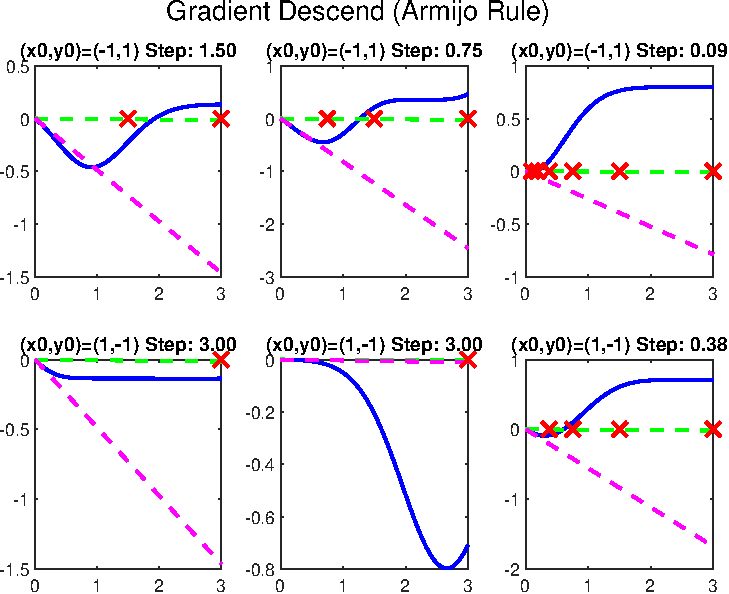
\includegraphics[width=1\linewidth]{plot/gradient_descend_armijo_rule_iters.pdf}
    \caption{Μέθοδος \selectlanguage{english} Armijo \selectlanguage{greek} για τις τρεις πρώτες επαναλήψεις της μεθόδου Μέγιστης Καθόδου}
    \label{fig:gradient_descend_armijo_rule_iters}
\end{figure}

\begin{figure}[h]
    \centering
    \begin{minipage}{0.47\textwidth}
        \centering
        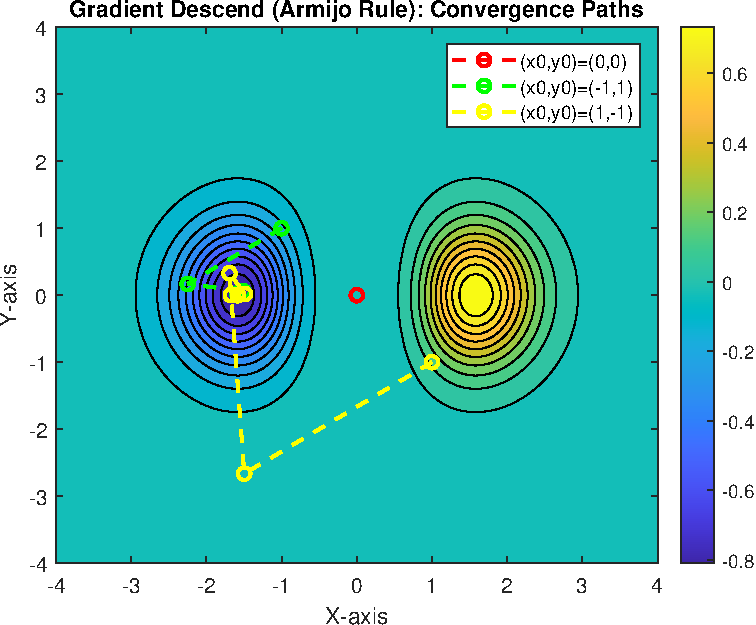
\includegraphics[width=1\linewidth]{plot/gradient_descend_armijo_rule_contour.pdf}
        \caption{\small Διαδοχικά σημεία υπολογισμού της μεθόδου Μέγιστης Καθόδου για βήμα μέσω του κανόνα \selectlanguage{english} Armijo \selectlanguage{greek}}
        \label{fig:gradient_descend_armijo_rule_contour}
    \end{minipage} \hfill
    \begin{minipage}{0.47\textwidth}
        \centering
        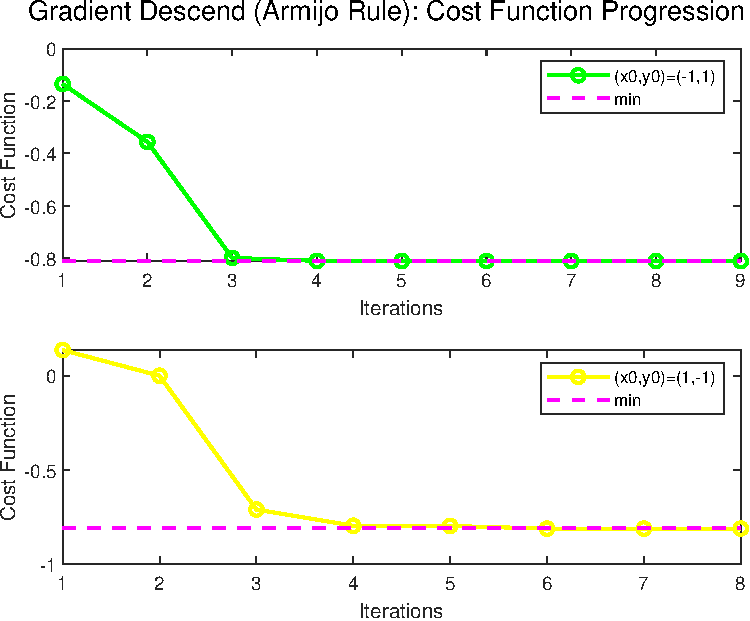
\includegraphics[width=1\linewidth]{plot/gradient_descend_armijo_rule_costs.pdf}
        \caption{\small Σύγκλιση της μεθόδου Μέγιστης Καθόδου για βήμα μέσω του κανόνα \selectlanguage{english} Armijo \selectlanguage{greek}}
        \label{fig:gradient_descend_armijo_rule_costs}
    \end{minipage}
\end{figure}


\section*{Μέθοδος \selectlanguage{english} Newton}
Σε αυτή τη μέθοδο, το διάνυσμα κατεύθυνσης $d_k$ επιλέγεται ως 
\[d_k = -\frac{[\nabla^2 f(x_k)]^{-1} \nabla f(x_k)}{|[\nabla^2 f(x_k)]^{-1} \nabla f(x_k)|}\]
όπου $\nabla^2 f(x_k)$ ο εσσιανός πίνακας της αντικειμενικής συνάρτησης. Η κανονικοποίηση του $d_k$ 
γίνεται για τους λόγους που αναφέρθηκαν παραπάνω. 

Επειδή η συγκεκριμένη μέθοδος λαμβάνει υπ' όψιν
την κυρτότητα της συνάρτησης επιτυγχάνει ταχύτερη σύγκλιση σε σχέση με την μέθοδο της μέγιστης καθόδου.
Ωστόσο αυτή η επιτάχυνση έρχεται και με μεγαλύτερο υπολογιστικό κόστος λόγω του υπολογισμού του αντίστροφου
του εσσιανού πίνακα. Ένα άλλο μειονέκτημα της μεθόδου είναι η απαίτηση ο εσσιανος πίνακας να είναι θετικά 
ορισμένος ώστε να μπορέσει να συγκλίνει στο ολικό ελάχιστο. 

Αυτός είναι και ο λόγος που στην περίπτωσή μας
ο αλγόριθμος αποτυγχάνει για τα αρχικά σημεία $(-1, 1)$, $(1, -1)$. Στο Σχήμα~\ref{fig:newton_fixed_step_contour}
έως Σχήμα~\ref{fig:newton_armijo_rule_costs} φαίνεται η απόκλιση του αλγορίθμου για κάθε περίπτωση υπολογισμού
του βήματος.

\begin{figure}[h]
    \centering
    \begin{minipage}{0.47\textwidth}
        \centering
        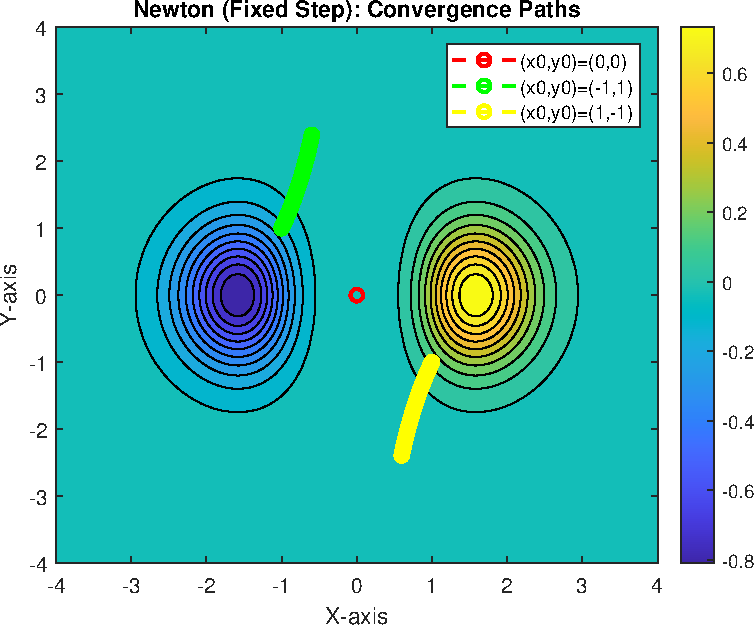
\includegraphics[width=1\linewidth]{plot/newton_fixed_step_contour.pdf}
        \caption{\small Διαδοχικά σημεία υπολογισμού της μεθόδου \selectlanguage{english} Newton \selectlanguage{greek} για σταθερό βήμα}
        \label{fig:newton_fixed_step_contour}
    \end{minipage} \hfill
    \begin{minipage}{0.47\textwidth}
        \centering
        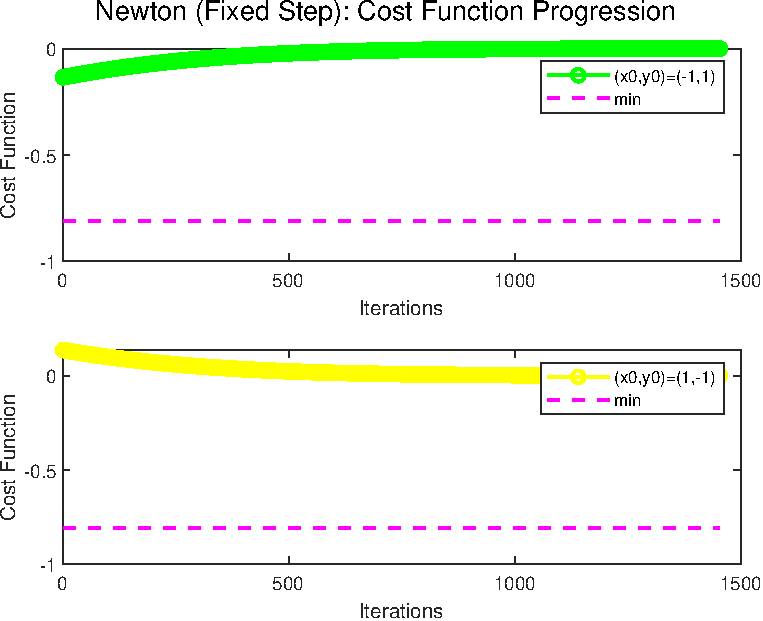
\includegraphics[width=1\linewidth]{plot/newton_fixed_step_costs.pdf}
        \caption{\small Σύγκλιση της μεθόδου \selectlanguage{english} Newton \selectlanguage{greek} για σταθερό βήμα}
        \label{fig:newton_fixed_step_costs}
    \end{minipage}
\end{figure}

\begin{figure}[h]
    \centering
    \begin{minipage}{0.47\textwidth}
        \centering
        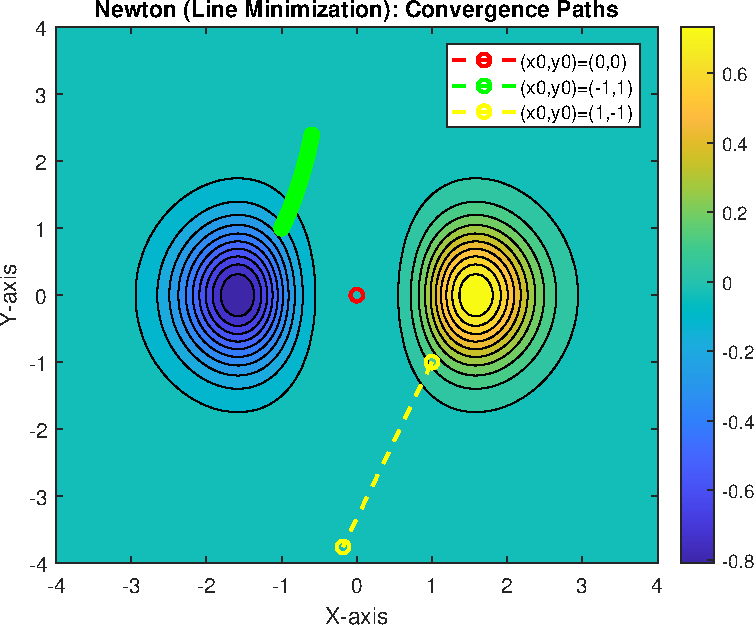
\includegraphics[width=1\linewidth]{plot/newton_line_minimization_contour.pdf}
        \caption{\small Διαδοχικά σημεία υπολογισμού της μεθόδου \selectlanguage{english} Newton \selectlanguage{greek} για βήμα μέσω ελαχιστοποίησης}
        \label{fig:newton_line_minimization_contour}
    \end{minipage} \hfill
    \begin{minipage}{0.47\textwidth}
        \centering
        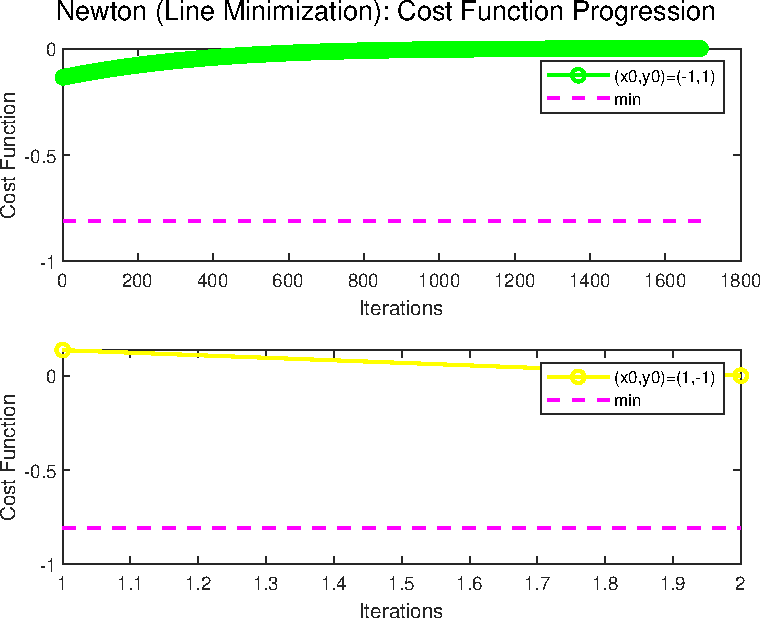
\includegraphics[width=1\linewidth]{plot/newton_line_minimization_costs.pdf}
        \caption{\small Σύγκλιση της μεθόδου \selectlanguage{english} Newton \selectlanguage{greek} για βήμα μέσω ελαχιστοποίησης}
        \label{fig:newton_line_minimization_costs}
    \end{minipage}
\end{figure}

\begin{figure}[h]
    \centering
    \begin{minipage}{0.47\textwidth}
        \centering
        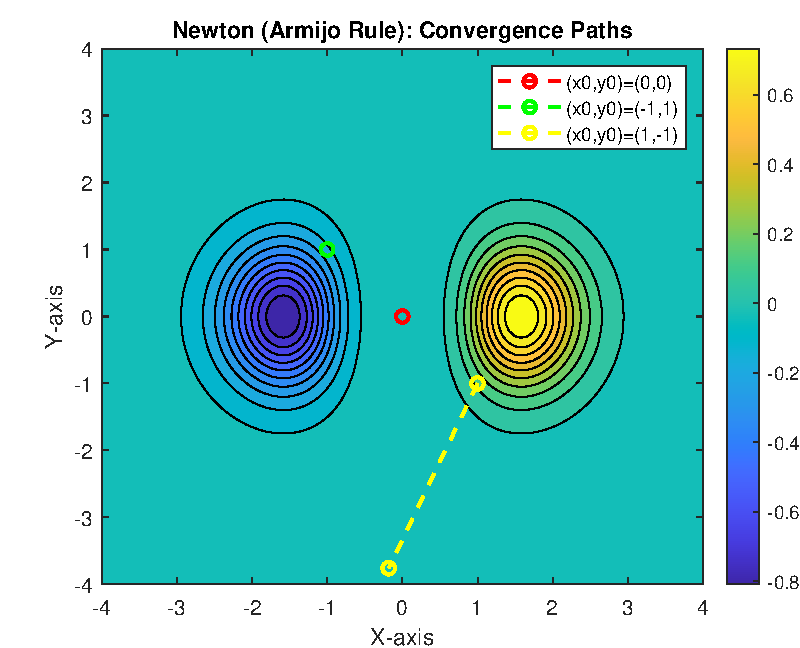
\includegraphics[width=1\linewidth]{plot/newton_armijo_rule_contour.pdf}
        \caption{\small Διαδοχικά σημεία υπολογισμού της μεθόδου \selectlanguage{english} Newton \selectlanguage{greek} για βήμα μέσω του κανόνα \selectlanguage{english} Armijo \selectlanguage{greek}}
        \label{fig:newton_armijo_rule_contour}
    \end{minipage} \hfill
    \begin{minipage}{0.47\textwidth}
        \centering
        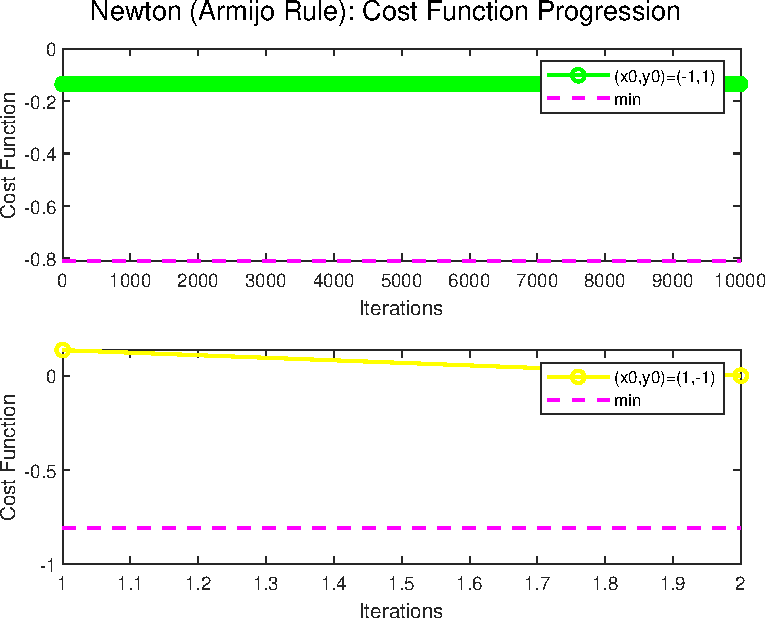
\includegraphics[width=1\linewidth]{plot/newton_armijo_rule_costs.pdf}
        \caption{\small Σύγκλιση της μεθόδου \selectlanguage{english} Newton \selectlanguage{greek} για βήμα μέσω του κανόνα \selectlanguage{english} Armijo \selectlanguage{greek}}
        \label{fig:newton_armijo_rule_costs}
    \end{minipage}
\end{figure}

\section*{Μέθοδος \selectlanguage{english} Levenberg-Marquardt}
Σε αυτή τη μέθοδο, το διάνυσμα κατεύθυνσης $d_k$ επιλέγεται ως 
\[d_k = -\frac{[\nabla^2 f(x_k) + \mu_k I]^{-1} \nabla f(x_k)}{|[\nabla^2 f(x_k) + \mu_k I]^{-1} \nabla f(x_k)|}.\]
Η κανονικοποίηση του $d_k$ γίνεται για λόγους που έχουν ήδη αναφερθεί. Αυτή η μέθοδος συνδυάζει την
ευρωστία της μεθόδου μέγιστης καθόδου με την ταχύτητα σύγκλισης της της μεθόδου\selectlanguage{english} Newton.
\selectlanguage{greek} 

Το πρόβλημα της απαίτησης για θετικά ορισμένο εσσιανό πίνακα στην μέθοδο\selectlanguage{english}
Newton\selectlanguage{greek} αίρεται με την κατάληλλη επιλογή του $\mu_k$. Πιο συγκεκριμένα όταν ο $\nabla^2 f(x_k)$ 
δεν είναι θετικά ορισμένος, υπολογίζουμε το $\mu_k$ έτσι ώστε ο πίνακας $\nabla^2 f(x_k) + \mu_k I$ να είναι θετικά 
ορισμένος. Αποδικνύεται ότι αυτό ισχύει όταν το $\mu_k$ είναι μεγαλύτερο από την μέγιστη κατ' απόλυτη τιμή ιδιοτιμή του
$\nabla^2 f(x_k)$. 

Το $\mu_k$ διαδραματίζει καθοριστίκο ρόλο στην συμπεριφορά του αλγορίθμου. Όταν $\mu_k \to 0$ 
ο όρος $\nabla^2 f(x_k)$ επικρατεί έναντι του $\mu_k I$ και η μέθοδος έχει παρόμοια συμπεριφορά με την μέθοδο 
\selectlanguage{english}Newton\selectlanguage{greek}. Αντίστοιχα όταν $\mu_k \to \infty$ ο όρος $\mu_k I$ επικρατεί
έναντι του $\nabla^2 f(x_k)$ και η μέθοδος έχει συμπεριφορά παρόμοια με αυτή της μέγιστης καθόδου. 

Στην ανάλυσή μας το $\mu_k$ επιλέγεται να είναι ίσο με την μέγιστη κατ' απόλυτη τιμή ιδιοτιμή του $\nabla^2 f(x_k)$ 
πολλαπλασιασμένη με μία σταθερά ελαφρώς μεγαλύτερη της μονάδας. Με αυτόν τον τρόπο έχουμε εγγυημένη σύγκλιση, 
ενώ εξασφαλίζουμε τη βέλτιστη δυνατή ταχύτητα σύγκλισης.

\subsection*{Σταθερό βήμα}
Στο Σχήμα~\ref{fig:levenberg_marquardt_fixed_step_contour} φαίνονται τα διαδοχικά σημεία που υπολογίζει ο αλγόριθμος σε 
κάθε επανάληψη για $\gamma_k = 0.001$. Παρόμοια με τη μέθοδο μέγιστης καθόδου, ο αλγόριθμος αποτυγχάνει να συγκλίνει
όταν το αρχικό σημείο είναι $(1, -1)$. 

Αυτό συμβαίνει επειδή, όταν ο αλγόριθμος βρίσκεται μακριά από το ελάχιστο, η συμπεριφορά του πλησιάζει εκείνη της
μεθόδου μέγιστης καθόδου. Στη μέθοδο αυτή, η κατεύθυνση της κίνησης εξαρτάται αποκλειστικά από την κλίση της
αντικειμενικής συνάρτησης, η οποία είναι περίπου μηδενική στην εν λόγω επιφάνεια, οδηγώντας σε αδυναμία βελτίωσης.

Εάν επιχειρήσουμε να αυξήσουμε το μέγεθος του βήματος ώστε να αποφύγουμε την επίπεδη περιοχή, αυτό οδηγεί σε αδυναμία 
σύγκλισης για τα δύο αρχικά σημεία λόγω ταλαντώσεων γύρω από το σημείο ισορροπίας. Επιπλέον, παρατηρούμε ότι, μετά 
από έναν αριθμό επαναλήψεων, η πορεία του σημείου $(-1, 1)$ προς το ελάχιστο παύει να είναι κάθετη στις ισοδυναμικές 
επιφάνειες. 

Αυτό συμβαίνει διότι, καθώς πλησιάζουμε στο ελάχιστο, η συμπεριφορά του αλγορίθμου προσεγγίζει εκείνη της μεθόδου 
\selectlanguage{english} Newton \selectlanguage{greek}, όπου η κυρτότητα της συνάρτησης καθοδηγεί τη λύση, αντί της
κλίσης, επιτρέποντας την εύρεση συντομότερης διαδρομής προς το ελάχιστο.

Στο Σχήμα~\ref{fig:levenberg_marquardt_fixed_step_costs} φαίνεται το κόστος συναρτήσει των επαναλήψεων. Παρατηρούμε
ότι η μέθοδος \selectlanguage{english} Levenberg-Marquardt \selectlanguage{greek} συγκλίνει ταχύτερα από την μέθοδο 
μέγιστης καθόδου όταν το βήμα είναι σταθερό, για τους λόγους που αναφέρθηκαν.


\begin{figure}[h]
    \centering
    \begin{minipage}{0.47\textwidth}
        \centering
        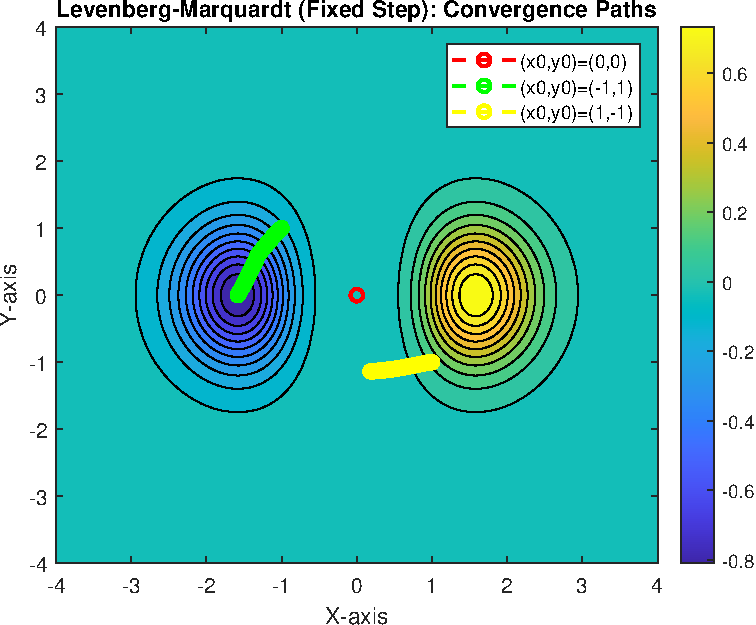
\includegraphics[width=1\linewidth]{plot/levenberg_marquardt_fixed_step_contour.pdf}
        \caption{\small Διαδοχικά σημεία υπολογισμού της μεθόδου\selectlanguage{english} Levenberg-Marquardt\selectlanguage{greek} για σταθερό βήμα $\gamma_k=0.001$}
        \label{fig:levenberg_marquardt_fixed_step_contour}
    \end{minipage} \hfill
    \begin{minipage}{0.47\textwidth}
        \centering
        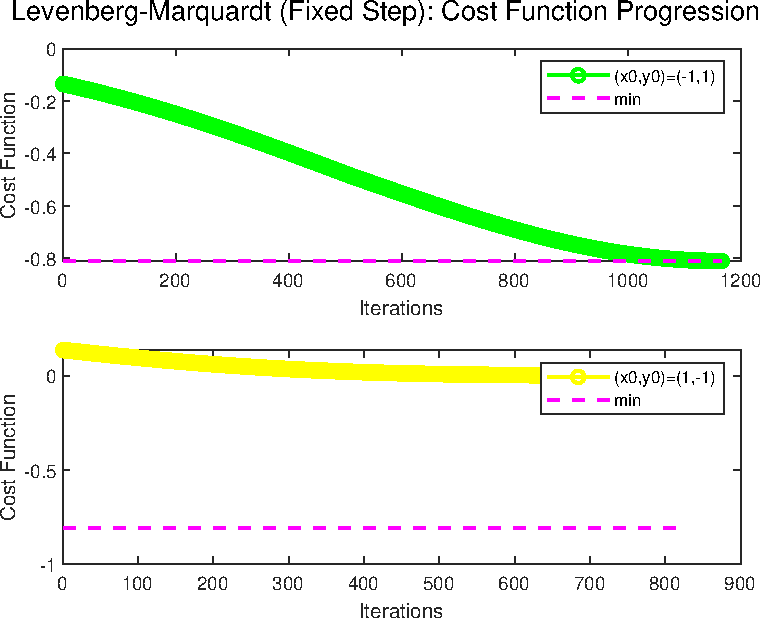
\includegraphics[width=1\linewidth]{plot/levenberg_marquardt_fixed_step_costs.pdf}
        \caption{\small Σύγκλιση της μεθόδου\selectlanguage{english} Levenberg-Marquardt\selectlanguage{greek} για σταθερό βήμα $\gamma_k=0.001$}
        \label{fig:levenberg_marquardt_fixed_step_costs}
    \end{minipage}
\end{figure}

\subsection*{Βήμα με ελαχιστοποίηση}
Στο Σχήμα~\ref{fig:levenberg_marquardt_line_minimization_contour} βλέπουμε τα διαδοχικά σημεία που υπολογίζει
ο αλγόριθμος \selectlanguage{english} Levenberg-Marquardt \selectlanguage{greek} με βήμα $\gamma_k$ που να
ελαχιστοποιεί την $f(x_k + \gamma_k d_k)$. Το διάστημα αναζήτησης ελαχίστου, όπως και στην μέθοδο μέγιστης καθόδου,
είναι $d=3$ ώστε να αποφύγουμε την επίπεδη περιοχή. Η ελαχιστοποίηση γίνεται και πάλι με την μέθοδο
\selectlanguage{english} Fibonacci \selectlanguage{greek}.

Στο Σχήμα~\ref{fig:levenberg_marquardt_line_minimization_costs} απεικονίζεται η σύγκλιση της μεθόδου σε κάθε επανάληψη 
για την περίπτωση ελαχιστοποίησης συνάρτησης. Παρατηρούμε ότι η μέθοδος κατέληξε στη λύση μέσα σε μόλις τέσσερις 
επανάληψεις για τα αρχικά σημεία $(-1, 1)$ και $(1, -1)$. Σε σύγκριση, η μέθοδος μέγιστης καθόδου απαιτούσε οκτώ 
επαναλήψεις για το σημείο $(-1, 1)$ και δέκα επαναλήψεις για το σημείο $(1, -1)$, αναδεικνύοντας την ταχύτερη 
σύγκλιση της παρούσας μεθόδου.

Όπως έχουμε ήδη αναφέρει, καθώς ο αλγόριθμος πλησιάζει στο ελάχιστο, η συμπεριφορά του αρχίζει να προσομοιάζει αυτήν της
μεθόδου \selectlanguage{english}Newton\selectlanguage{greek}. Σε αυτό το στάδιο, η πορεία προς τη λύση καθορίζεται
κυρίως από την κυρτότητα της συνάρτησης αντί για την κλίση, επιτρέποντας την επιλογή μιας πιο αποτελεσματικής και άμεσης
διαδρομής προς το ελάχιστο.

\begin{figure}[h]
    \centering
    \begin{minipage}{0.47\textwidth}
        \centering
        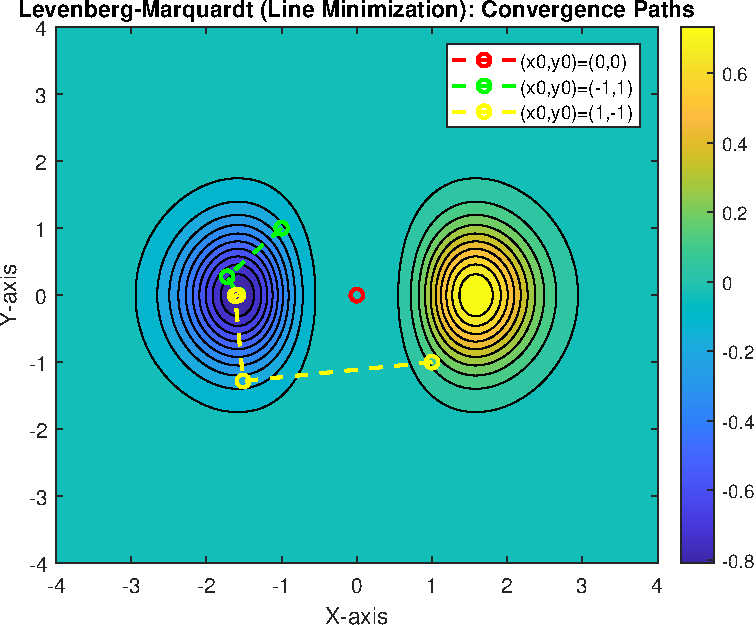
\includegraphics[width=1\linewidth]{plot/levenberg_marquardt_line_minimization_contour.pdf}
        \caption{\small Διαδοχικά σημεία υπολογισμού της μεθόδου \selectlanguage{english} Levenberg-Marquardt \selectlanguage{greek} για βήμα μέσω ελαχιστοποίησης}
        \label{fig:levenberg_marquardt_line_minimization_contour}
    \end{minipage} \hfill
    \begin{minipage}{0.47\textwidth}
        \centering
        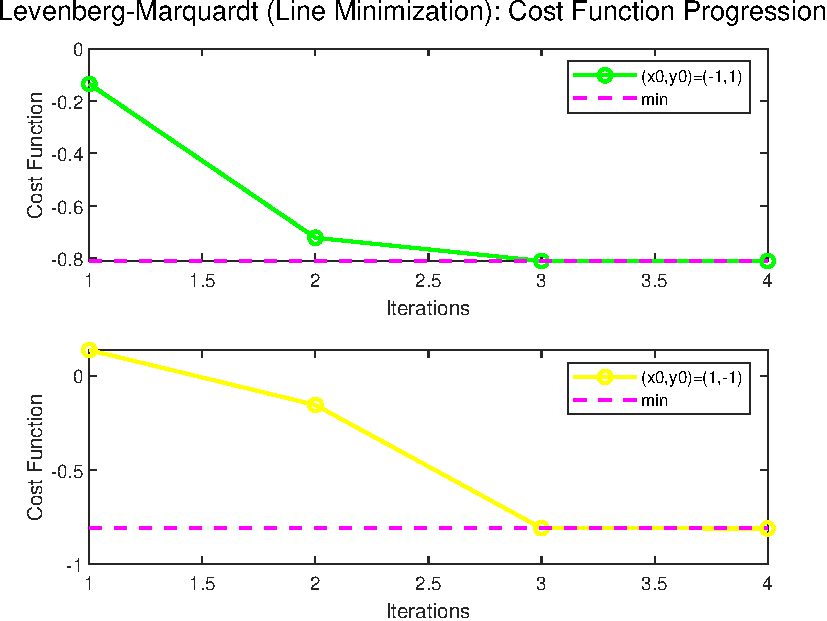
\includegraphics[width=1\linewidth]{plot/levenberg_marquardt_line_minimization_costs.pdf}
        \caption{\small Σύγκλιση της μεθόδου \selectlanguage{english} Levenberg-Marquardt \selectlanguage{greek} για βήμα μέσω ελαχιστοποίησης}
        \label{fig:levenberg_marquardt_line_minimization_costs}
    \end{minipage}
\end{figure}

\subsection*{Βήμα με τον κανόνα \selectlanguage{english} Armijo}
\selectlanguage{greek}
Στο Σχήμα~\ref{fig:levenberg_marquardt_armijo_rule_iters} παρουσιάζονται οι τρεις πρώτες επαναλήψεις της μεθόδου 
\selectlanguage{english} Armijo \selectlanguage{greek} για τα αρχικά σημεία $(-1, 1)$ και $(1, -1)$,
με παραμέτρους $s = 3$, $\beta = 0.5$, και $\alpha = 0.01$. Οι τιμές των παραμέτρων επιλέχθηκαν όπως και στην 
μέθοδο μέγιστης καθόδου για τους λόγους που έχουν είδη αναφερθεί.

Από το Σχήμα~\ref{fig:levenberg_marquardt_line_minimization_costs}
και το Σχήμα~\ref{fig:levenberg_marquardt_armijo_rule_costs} παρατηρούμε ότι η μέθοδος 
\selectlanguage{english} Levenberg-Marquardt \selectlanguage{greek} συγκλίνει πιο αργά όταν χρησιμοποιείται ο κανόνας
\selectlanguage{english} Armijo \selectlanguage{greek}, σε σχέση με την περίπτωση της ελαχιστοποίησης της συνάρτησης 
$f(x_k + \gamma_k d_k)$. Αυτό μπορεί να εξηγηθεί, καθώς στην περίπτωση της ελαχιστοποίησης της συνάρτησης επιτυγχάνεται
η μέγιστη δυνατή βελτίωση σε κάθε βήμα.

Επίσης, από το Σχήμα~\ref{fig:gradient_descend_armijo_rule_costs}
και το Σχήμα~\ref{fig:levenberg_marquardt_armijo_rule_costs} βλέπουμε ότι για αρχικό σημείο το $(-1, 1)$
οι δύο μέθοδοι απαιτούν τον ίδιο αριθμό επαναλήψεων ενώ για αρχικό σημείο το $(1, -1)$ η μέθοδος
\selectlanguage{english}Levenberg-Marquardt\selectlanguage{greek} παρουσιάζει πιο αργή σύγκλιση σε σχέση με την
μέθοδο μέγιστης καθόδου.

\begin{figure}
    \centering
    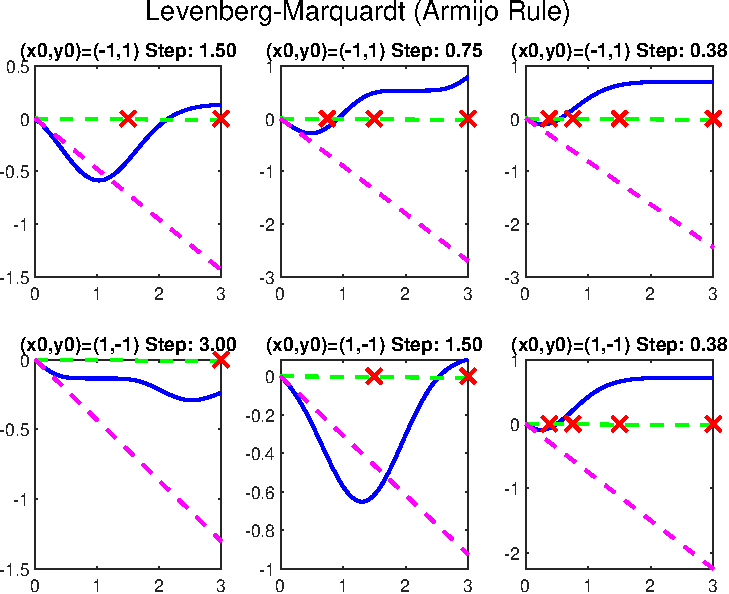
\includegraphics[width=1\linewidth]{plot/levenberg_marquardt_armijo_rule_iters.pdf}
    \caption{Μέθοδος \selectlanguage{english} Armijo \selectlanguage{greek} για τις τρεις πρώτες επαναλήψεις της μεθόδου \selectlanguage{english} Levenberg-Marquardt \selectlanguage{greek}}
    \label{fig:levenberg_marquardt_armijo_rule_iters}
\end{figure}

\begin{figure}[h]
    \centering
    \begin{minipage}{0.47\textwidth}
        \centering
        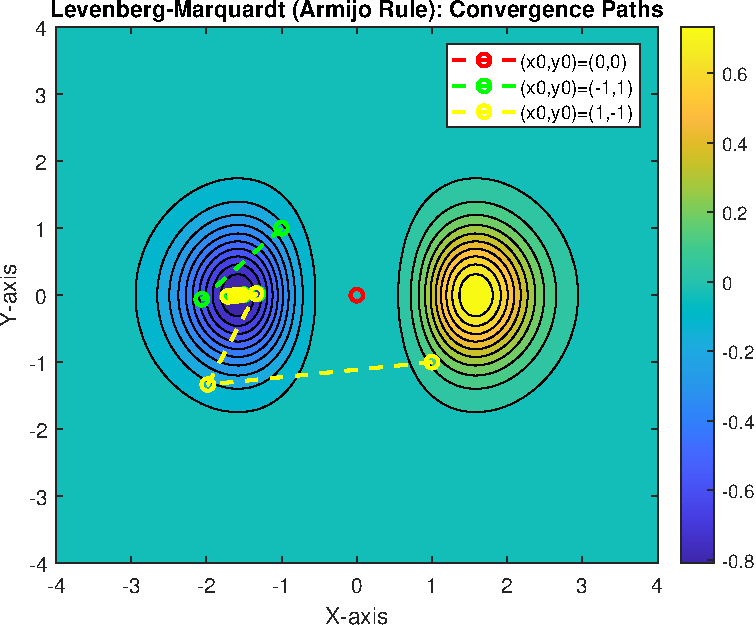
\includegraphics[width=1\linewidth]{plot/levenberg_marquardt_armijo_rule_contour.pdf}
        \caption{\small Διαδοχικά σημεία υπολογισμού της μεθόδου \selectlanguage{english} Levenberg-Marquardt \selectlanguage{greek} για βήμα μέσω του κανόνα \selectlanguage{english} Armijo \selectlanguage{greek}}
        \label{fig:levenberg_marquardt_armijo_rule_contour}
    \end{minipage} \hfill
    \begin{minipage}{0.47\textwidth}
        \centering
        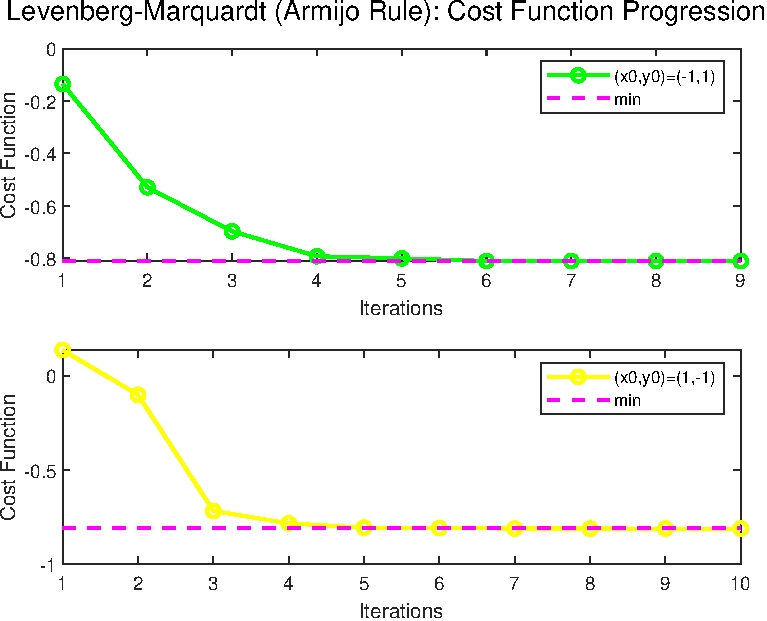
\includegraphics[width=1\linewidth]{plot/levenberg_marquardt_armijo_rule_costs.pdf}
        \caption{\small Σύγκλιση της μεθόδου \selectlanguage{english} Levenberg-Marquardt \selectlanguage{greek} για βήμα μέσω του κανόνα \selectlanguage{english} Armijo \selectlanguage{greek}}
        \label{fig:levenberg_marquardt_armijo_rule_costs}
    \end{minipage}
\end{figure}


\section*{Συμπέρασμα}

Συμπερασματικά, η επιλογή του σημείου εκκίνησης και του βήματος $\gamma_k$ επηρεάζει σημαντικά τη συμπεριφορά των
μεθόδων βελτιστοποίησης. Στη μέθοδο μέγιστης καθόδου, ένα κακό σημείο εκκίνησης μπορεί να οδηγήσει σε αργή σύγκλιση, 
ιδίως αν βρίσκεται σε επίπεδες περιοχές. Επιπλέον, η χρήση σταθερού $\gamma_k$ ενδέχεται να μην προσαρμόζεται στις 
αλλαγές της γεωμετρίας του προβλήματος, καθυστερώντας τη σύγκλιση, ενώ η προσαρμοστική επιλογή $\gamma_k$, π.χ. μέσω 
ελαχιστοποίησης της κατεύθυνσης ή κανόνα \selectlanguage{english}Armijo\selectlanguage{greek}, επιταχύνει τη
διαδικασία. Στη μέθοδο \selectlanguage{english}Newton\selectlanguage{greek}, το σημείο εκκίνησης επηρεάζει την
εγγύτητα προς τη σύγκλιση, ενώ οι κακές αρχικές επιλογές μπορεί να οδηγήσουν σε μη θετικούς ορισμένους εσσιανούς ή σε 
αποκλίσεις. Η μέθοδος \selectlanguage{english}Levenberg-Marquardt\selectlanguage{greek} ξεπερνά τέτοια προβλήματα με
την προσθήκη όρου απόσβεσης, καθιστώντας τη πιο ανεκτική σε απομακρυσμένα σημεία εκκίνησης. Συνολικά, οι μέθοδοι που 
ρυθμίζουν δυναμικά το $\gamma_k$ αποδείχθηκαν πιο αποτελεσματικές, εξισορροπώντας την ταχύτητα και την ακρίβεια της 
σύγκλισης, ιδιαίτερα όταν το σημείο εκκίνησης βρίσκεται μακριά από το ολικό ελάχιστο.

\end{document}
